%(BEGIN_QUESTION)
% Copyright 2006, Tony R. Kuphaldt, released under the Creative Commons Attribution License (v 1.0)
% This means you may do almost anything with this work of mine, so long as you give me proper credit

Velg passende motstandsverdier slik at op-ampen gir et spenningssignal fra 0 til 5 volt over et temperaturmåleområde fra 0$^{o}$ C til 80$^{o}$ C. Anta bruk av en 1000 $\Omega$ RTD med europeisk alpha.

$$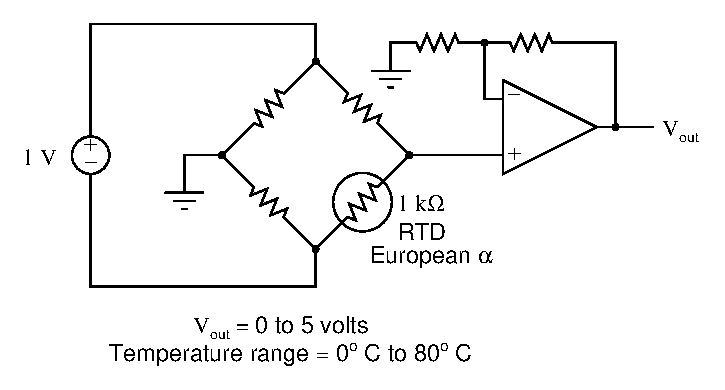
\includegraphics[width=15.5cm]{i00411x01.eps}$$

\vskip 20pt \vbox{\hrule \hbox{\strut \vrule{} {\bf Forslag til sokratisk diskusjon} \vrule} \hrule}

\begin{itemize}
\item{} Påvirker de to tilbakekoblingsmotstandene i operasjonsforsterkeren kretsens {\it nullpunkt}, {\it spennvidde} eller {\it linearitet}?
\item{} Hvordan kan vi legge til {\it justerbar} nullpunkt- og spennviddekalibrering i denne kretsen?
\item{} Velg en vilkårlig motstand i kretsen og tenk at den feiler (enten avbrudd eller kortslutning). Vil denne elektriske feilen få RTD-en til å se varmere ut enn den faktisk er, eller kaldere? Forklar svaret i detalj.
\end{itemize}

\underbar{file i00411}
%(END_QUESTION)





%(BEGIN_ANSWER)

Ved 0 grader C er $R_{RTD}$ = 1000 $\Omega$ og $V_{+}$ = 0 volt.

\vskip 10pt

Ved 80 grader C er $R_{RTD}$ = 1308 $\Omega$ og $V_{+}$ = 0.06672 volt (forutsatt at alle de andre motstandene i broen er 1 k$\Omega$ hver).

\vskip 10pt

For å få 5 volt ut fra op-ampen med 66.72 mV inn trenger vi en spenningsforsterkning på nøyaktig 74.935. Siden op-amp-kretsen er ikke-inverterende, og spenningsforsterkningen er forholdet mellom tilbakekoblingsmotstandene pluss én, trenger vi et motstandsforhold på 73.935:1.

\vskip 10pt

Følgende motstandsverdier foreslås, men dette er ikke de {\it eneste} riktige verdiene som kan gi samme kalibrering:

$$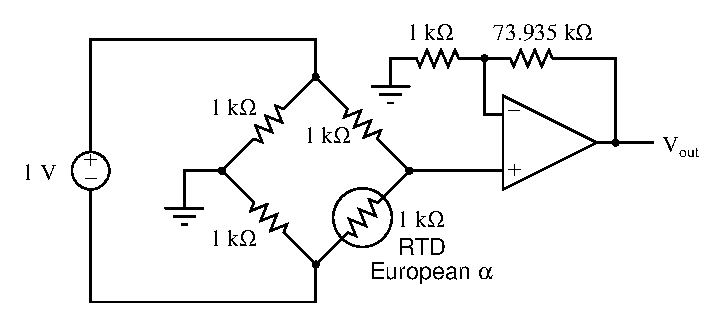
\includegraphics[width=15.5cm]{i00411x02.eps}$$

%(END_ANSWER)





%(BEGIN_NOTES)








\vskip 20pt \vbox{\hrule \hbox{\strut \vrule{} {\bf Virtuell feilsøking} \vrule} \hrule}

Dette spørsmålet egner seg godt som en «virtuell feilsøking»-øvelse. Når du presenterer kretsdiagrammet for studentene, ser du først for deg en bestemt feil i systemet. Deretter presenterer du ett eller flere symptomer på denne feilen (noe en operatør eller annen bruker kan observere). Studentene foreslår så ulike diagnostiske tester for å identifisere feiltype og feilsted, som om de var teknikere som feilsøkte systemet. Din oppgave er å fortelle hva resultatet ville blitt for hver foreslåtte test, og dokumentere resultatene slik at alle studentene kan se dem.

Under og etter øvelsen er det nyttig å stille oppfølgingsspørsmål som:

\begin{itemize}
\item{} Hva forteller resultatet av den siste diagnostiske testen om feilen?
\item{} Anta at resultatet av den siste testen hadde vært annerledes. Hva ville det i så fall fortalt om feilen?
\item{} Er den siste diagnostiske testen den beste vi kunne gjort?
\item{} Hva ville vært den ideelle testrekkefølgen for å finne feilen i færrest mulig trinn?
\end{itemize}


%INDEX% Measurement, temperature: RTD

%(END_NOTES)
